% ---------------------------------------------------------------- 20 Augmentation
\begin{frame}{Augmentation is the regularizer}
  \small
  One scene is the whole dataset, so the regularizer matters more than usual. The
  candidate transforms, screened by acquisition geometry:
  \begin{center}
  \begin{tikzpicture}
    \begin{scope}
      \node[font=\tiny\bfseries,anchor=south] at (0.6,1.32) {original patch};
      \draw[soft,thin,fill=white] (0,0) rectangle (1.2,1.2);
      \draw[black!10,step=0.3] (0,0) grid (1.2,1.2);
      \fill[accent!70] (0.25,0.25) -- (0.85,0.25) -- (0.25,0.85) -- cycle;
      \draw[->,soft] (-0.22,0) -- (-0.22,1.2);
      \node[font=\tiny,soft,anchor=east] at (-0.26,0.6) {rg};
      \draw[->,soft] (0,-0.22) -- (1.2,-0.22);
      \node[font=\tiny,soft,anchor=north] at (0.6,-0.28) {az};
    \end{scope}
    \draw[flow] (1.6,0.6) -- (2.2,0.6);
    \draw[good!60,thick,rounded corners=3pt,fill=good!5] (2.25,-0.3) rectangle (6.4,1.78);
    \node[font=\tiny,good,anchor=north] at (4.33,-0.42)
      {\textbf{axis preserving --- used} ($p{=}0.5$ each)};
    \begin{scope}[xshift=2.5cm]
      \node[font=\tiny\bfseries,anchor=south] at (0.6,1.32) {flip azimuth};
      \draw[soft,thin,fill=white] (0,0) rectangle (1.2,1.2);
      \draw[black!10,step=0.3] (0,0) grid (1.2,1.2);
      \fill[accent!70] (0.95,0.25) -- (0.35,0.25) -- (0.95,0.85) -- cycle;
    \end{scope}
    \begin{scope}[xshift=4.95cm]
      \node[font=\tiny\bfseries,anchor=south] at (0.6,1.32) {flip range};
      \draw[soft,thin,fill=white] (0,0) rectangle (1.2,1.2);
      \draw[black!10,step=0.3] (0,0) grid (1.2,1.2);
      \fill[accent!70] (0.25,0.95) -- (0.85,0.95) -- (0.25,0.35) -- cycle;
    \end{scope}
    \draw[accent!60,thick,rounded corners=3pt,fill=accent!5] (7.15,-0.3) rectangle (8.85,1.78);
    \node[font=\tiny,accent,anchor=north] at (8.0,-0.42)
      {\textbf{axis swapping --- not used}};
    \begin{scope}[xshift=7.4cm]
      \node[font=\tiny\bfseries,anchor=south] at (0.6,1.32) {rotate $90^\circ$};
      \draw[soft,thin,fill=white] (0,0) rectangle (1.2,1.2);
      \draw[black!10,step=0.3] (0,0) grid (1.2,1.2);
      \fill[accent!70] (0.25,0.95) -- (0.25,0.35) -- (0.85,0.95) -- cycle;
    \end{scope}
  \end{tikzpicture}
  \end{center}
  \begin{columns}[c]
    \begin{column}{0.52\textwidth}
      \begin{itemize}
        \item Flips are applied \textbf{jointly to input and target} ($p{=}0.5$ each):
              four orientations of every patch, spatial correspondence intact --- and
              each axis keeps its physical identity.
        \item Rotation would exchange range and azimuth --- two physically distinct
              axes (resolution, acquisition geometry, statistics) --- so only the
              axis-preserving pair is used.
      \end{itemize}
    \end{column}
    \begin{column}{0.46\textwidth}
      \centering
      \begin{tikzpicture}
        \draw[->,soft] (0,0) -- (4.6,0) node[right,font=\tiny]{epoch};
        \draw[->,soft] (0,0) -- (0,2.15) node[above,font=\tiny]{loss};
        \draw[soft!70,thick] plot[smooth] coordinates
          {(0.15,1.9) (0.8,1.0) (1.6,0.62) (2.4,0.45) (3.2,0.36) (4.1,0.29)};
        \draw[accent,thick,dashed] plot[smooth] coordinates
          {(0.15,1.95) (0.8,1.15) (1.4,0.95) (2.0,1.05) (2.8,1.32) (4.1,1.72)};
        \draw[good,thick] plot[smooth] coordinates
          {(0.15,1.95) (0.8,1.1) (1.6,0.8) (2.4,0.66) (3.2,0.58) (4.1,0.53)};
        \draw[soft,dashed,thin] (1.4,0) -- (1.4,2.05);
        \node[font=\tiny,accent,anchor=south west] at (1.45,1.85) {early overfit, no flips};
        \node[font=\tiny,soft,anchor=west]   at (4.2,0.29) {train};
        \node[font=\tiny,good,anchor=west]   at (4.2,0.53) {val, flips};
        \node[font=\tiny,accent,anchor=west] at (4.2,1.72) {val, no aug};
      \end{tikzpicture}
      \\[1pt]
      {\scriptsize The flips push the validation turn-off point out --- the single-scene
       overfit arrives much later.}
    \end{column}
  \end{columns}
\end{frame}

% ---------------------------------------------------------------- 20b Augmentation verdict
\begin{frame}{Augmentation, measured --- flips delay the overfit and halve the seed spread}
    \centering
  {\scriptsize
  \renewcommand{\arraystretch}{0.78}
  \setlength{\tabcolsep}{6pt}
  \renewcommand{\seedtag}{augA}
  \begin{tabular}{@{}lccr@{}}
    \toprule
    metric & no aug & flips & $\Delta$ \\
    \midrule
    \multicolumn{4}{@{}l}{\emph{training (single scene, validation)}} \\
    best epoch (val) & 26.2    & \hlval{good}{\textbf{43.8}}    & \hlval{good}{$+17.6$}    \\
    best val loss $\downarrow$  & \seedpm{0.1443}{.0008} & \seedpm{\hlval{good}{0.1420}}{.0007} & \hlval{good}{$-0.0023$} \\
    \addlinespace[1pt]
    \multicolumn{4}{@{}l}{\emph{reconstruction (curve)}} \\
    curve $R^2$ $\uparrow$     & \seedpm{0.573}{.022} & \seedpm{0.569}{.008} & \textcolor{soft}{$-0.004$} \\
    curve MAE $\downarrow$     & \seedpm{0.0501}{.0012} & \seedpm{0.0496}{.0008} & \textcolor{soft}{$-0.0005$} \\
    PSNR [dB] $\uparrow$       & \seedpm{50.36}{.22} & \seedpm{50.32}{.08} & \textcolor{soft}{$-0.04$}  \\
    per-pixel $R^2$ $\uparrow$ & \seedpm{0.359}{.050} & \seedpm{0.359}{.031} & \textcolor{soft}{$-0.001$} \\
    profile cos med $\uparrow$ & \seedpm{0.851}{.020} & \seedpm{0.850}{.024} & \textcolor{soft}{$-0.001$} \\
    SSIM elev $\uparrow$       & \seedpm{0.9582}{.0009} & \seedpm{0.9586}{.0006} & \textcolor{soft}{$+0.0004$} \\
    SSIM range $\uparrow$      & \seedpm{0.9257}{.0027} & \seedpm{0.9258}{.0021} & \textcolor{soft}{$+0.0002$} \\
    SSIM azim $\uparrow$       & \seedpm{0.9457}{.0014} & \seedpm{0.9461}{.0012} & \textcolor{soft}{$+0.0004$} \\
    peak err mean $\downarrow$ & \seedpm{\textbf{4.47}}{.86} & \seedpm{4.70}{.47} & \textcolor{soft}{$+0.23$}  \\
    \quad median $\downarrow$  & \seedpm{0.94}{.37} & \seedpm{\textbf{0.81}}{.30} & \textcolor{soft}{$-0.13$}  \\
    \quad p95 $\downarrow$     & \seedpm{15.44}{.67} & \seedpm{15.44}{.47} & \textcolor{soft}{$+0.00$}  \\
    \addlinespace[1pt]
    \multicolumn{4}{@{}l}{\emph{detection (matched)}} \\
    precision $\uparrow$       & \seedpm{0.816}{.015} & \seedpm{0.821}{.008} & \textcolor{soft}{$+0.005$}  \\
    recall $\uparrow$          & \seedpm{0.656}{.056} & \seedpm{0.641}{.029} & \textcolor{soft}{$-0.015$} \\
    matched F1 $\uparrow$      & \seedpm{0.727}{.040} & \seedpm{0.720}{.020} & \textcolor{soft}{$-0.007$} \\
    count exact $\uparrow$     & \seedpm{0.611}{.066} & \seedpm{0.595}{.034} & \textcolor{soft}{$-0.016$} \\
    \addlinespace[1pt]
    \multicolumn{4}{@{}l}{\emph{seed-to-seed spread (std over 5 seeds)} $\downarrow$} \\
    recall            & .056 & \hlval{good}{\textbf{.029}} & \hlval{good}{$-48\%$} \\
    count exact       & .066 & \hlval{good}{\textbf{.034}} & \hlval{good}{$-49\%$} \\
    peak err mean     & .86  & \hlval{good}{\textbf{.47}}  & \hlval{good}{$-46\%$} \\
    per-pixel $R^2$   & .050 & \hlval{good}{\textbf{.031}} & \hlval{good}{$-38\%$} \\
    \bottomrule
  \end{tabular}}
  \par\vspace{1pt}
  \parbox{0.82\textwidth}{\tiny\color{soft} \textbf{runs}: UNet $\cdot$ conv $\cdot$ sorted-GT $\cdot$ $K{=}2$ $\cdot$ param-MSE $\cdot$ presence none $\cdot$ full norm ladder $\cdot$ patch $64{\times}32$ (aug = column); cells: mean $\pm$ std over five seeds. Training rows: validation split; others: held-out test, $5.0$\,M px. \textbf{bold} = better mean, marked only where the two differ by more than $5\%$; $\Delta =$ flips $-$ no aug, coloured (\textcolor{good}{gain} / \textcolor{accent}{cost}) only where $|\Delta|$ clears it; spread rows compare the seed stds; \textcolor{good}{green values} $=$ the training shift and the spread halving --- the effects that clear it. Peak median/p95: per-pixel peak-error distribution; cos med: median profile cosine; peak in elevation units.\par}

\end{frame}

% ---------------------------------------------------------------- 20b2 Augmentation by scatterer count
\begin{frame}{Augmentation by scatterer count --- no accuracy shift, half the spread}
    \centering
  \scriptsize
  \renewcommand{\arraystretch}{1.08}
  \setlength{\tabcolsep}{6pt}
  \renewcommand{\seedtag}{augB}
  \begin{tabular}{@{}l c c r@{}}
    \toprule
    metric & no aug & flips & $\Delta$ \\
    \midrule
    matched precision $\uparrow$ & \seedpm{0.816}{.015} & \seedpm{0.821}{.008} & \textcolor{soft}{$+0.005$} \\
    \quad $k{=}1$                & \seedpm{0.848}{.019} & \seedpm{0.853}{.008} & \textcolor{soft}{$+0.005$} \\
    \quad $k{=}2$                & \seedpm{0.776}{.013} & \seedpm{0.782}{.007} & \textcolor{soft}{$+0.006$} \\
    \addlinespace
    matched recall $\uparrow$    & \seedpm{0.656}{.056} & \seedpm{0.641}{\hlval{good}{.029}} & \textcolor{soft}{$-0.015$} \\
    \quad $k{=}1$                & \seedpm{0.647}{.088} & \seedpm{0.620}{\hlval{good}{.046}} & \textcolor{soft}{$-0.028$} \\
    \quad $k{=}2$                & \seedpm{0.670}{.016} & \seedpm{0.672}{\hlval{good}{.008}} & \textcolor{soft}{$+0.002$} \\
    \addlinespace
    count acc $\mid$ pred $k{=}1$ $\uparrow$ & \seedpm{0.952}{.009} & \seedpm{0.948}{.007} & \textcolor{soft}{$-0.004$} \\
    count acc $\mid$ pred $k{=}2$ $\uparrow$ & \seedpm{0.720}{.013} & \seedpm{0.733}{.010} & \textcolor{soft}{$+0.013$} \\
    \addlinespace
    matched $\mu$ MAE $\downarrow$ & \seedpm{2.30}{.12} & \seedpm{2.30}{.08} & \textcolor{soft}{$+0.00$} \\
    \quad $k{=}1$                & \seedpm{0.63}{.06} & \seedpm{\textbf{0.59}}{.04} & \textcolor{soft}{$-0.04$} \\
    \quad $k{=}2$                & \seedpm{4.07}{.05} & \seedpm{4.05}{.08} & \textcolor{soft}{$-0.02$} \\
    \addlinespace
    matched $\sigma$ MAE $\downarrow$ & \seedpm{0.86}{.05} & \seedpm{0.87}{.03} & \textcolor{soft}{$+0.01$} \\
    \quad $k{=}1$                & \seedpm{0.25}{.02} & \seedpm{0.25}{.01} & \textcolor{soft}{$+0.00$} \\
    \quad $k{=}2$                & \seedpm{1.51}{.01} & \seedpm{1.51}{.01} & \textcolor{soft}{$+0.00$} \\
    \addlinespace
    matched $a$ MAE $\downarrow$ & \seedpm{0.364}{.034} & \seedpm{0.374}{.026} & \textcolor{soft}{$+0.010$} \\
    \quad $k{=}1$                & \seedpm{0.155}{.029} & \seedpm{0.161}{.017} & \textcolor{soft}{$+0.006$} \\
    \quad $k{=}2$                & \seedpm{0.586}{.035} & \seedpm{0.593}{.022} & \textcolor{soft}{$+0.007$} \\
    \bottomrule
  \end{tabular}
  \par\vspace{3pt}
  \parbox{0.82\textwidth}{\tiny\color{soft} \textbf{runs}: UNet $\cdot$ conv $\cdot$ sorted-GT $\cdot$ $K{=}2$ $\cdot$ param-MSE $\cdot$ presence none $\cdot$ full norm ladder $\cdot$ patch $64{\times}32$ (aug = column); held-out test band, cells mean $\pm$ seed std over five seeded replicas; $k$ $=$ true scatterer count of the pixel. \textbf{bold} $=$ better mean, marked only where the two differ by more than $5\%$; $\Delta$ $=$ flips $-$ no aug, coloured only where $|\Delta|$ clears it; \textcolor{good}{green} $\pm$ $=$ the spread halving --- the one effect that does. Precision rewards under-prediction --- rank on recall. count acc $\mid$ pred $k$: share of pixels claiming exactly $k$ scatterers whose true count is $k$. $\mu$, $\sigma$ in elevation units; $a$ in linear amplitude.\par}
    

\end{frame}

% ---------------------------------------------------------------- 20b3 Augmentation: predicted stats vs GT
\begin{frame}{Augmentation, predicted statistics vs the GT --- same calibration, pinned down}
    \centering
  \scriptsize
  \renewcommand{\arraystretch}{1.00}
  \setlength{\tabcolsep}{6pt}
  \renewcommand{\seedtag}{augC}
  \begin{tabular}{@{}l !{\color{white}\vrule width 2pt} c !{\color{white}\vrule width 2pt} c c r@{}}
    \toprule
    prediction mean & \textcolor{good}{GT} & no aug & flips & $\Delta$ \\
    \midrule
    \multicolumn{5}{@{}l}{\textcolor{soft}{\emph{slot 0 --- strongest scatterer; GT-active on every pixel}}} \\
    \quad active frac            & 1.00    & \seedpm{0.706}{.066} & \seedpm{0.685}{\hlval{good}{.035}} & \textcolor{soft}{$-0.021$} \\
    \quad $a$ --- active         & 0.77    & \seedpm{0.89}{.07}   & \seedpm{0.90}{.03}   & \textcolor{soft}{$+0.01$} \\
    \quad $\mu$ --- active       & $-4.89$ & \seedpm{$-4.03$}{.15} & \seedpm{$-3.92$}{\hlval{good}{.10}} & \textcolor{soft}{$+0.11$} \\
    \quad $\sigma$ --- active    & 1.76    & \seedpm{1.52}{.08}   & \seedpm{1.48}{.05}   & \textcolor{soft}{$-0.04$} \\
    \addlinespace
    \multicolumn{5}{@{}l}{\textcolor{soft}{\emph{slot 1 --- second scatterer; GT-active on 26\% of pixels}}} \\
    \quad active frac            & 0.260 & \seedpm{0.306}{.008} & \seedpm{0.299}{.006} & \textcolor{soft}{$-0.007$} \\
    \quad $a$ --- active         & 1.43  & \seedpm{1.06}{.05} & \seedpm{1.04}{.03} & \textcolor{soft}{$-0.02$} \\
    \quad $a$ --- inact.         & 0.00  & \seedpm{0.45}{.04} & \seedpm{\textbf{0.42}}{\hlval{good}{.01}} & \textcolor{soft}{$-0.03$} \\
    \quad $\mu$ --- active       & 11.34 & \seedpm{9.97}{.40} & \seedpm{10.09}{.33} & \textcolor{soft}{$+0.12$} \\
    \quad $\mu$ --- inact.       & ---   & \seedpm{3.39}{.57} & \seedpm{4.09}{.31} & \textcolor{soft}{$+0.70$} \\
    \quad $\sigma$ --- active    & 3.53  & \seedpm{3.02}{.04} & \seedpm{2.94}{.05} & \textcolor{soft}{$-0.08$} \\
    \quad $\sigma$ --- inact.    & ---   & \seedpm{1.90}{.04} & \seedpm{1.87}{.03} & \textcolor{soft}{$-0.03$} \\
    \addlinespace
    \multicolumn{5}{@{}l}{\textcolor{soft}{\emph{distribution width --- std over GT-active pixels}}} \\
    \quad $a$ --- slot 0         & 1.48  & \seedpm{1.17}{.06} & \seedpm{1.17}{.03} & \textcolor{soft}{$+0.01$} \\
    \quad $\mu$ --- slot 0       & 3.30  & \seedpm{2.03}{.12} & \seedpm{1.99}{.07} & \textcolor{soft}{$-0.04$} \\
    \quad $\sigma$ --- slot 0    & 2.84  & \seedpm{\textbf{1.01}}{.03} & \seedpm{\hlval{accent}{0.95}}{.03} & \hlval{accent}{$-0.06$} \\
    \quad $a$ --- slot 1         & 1.45  & \seedpm{0.84}{.05} & \seedpm{0.83}{.04} & \textcolor{soft}{$-0.01$} \\
    \quad $\mu$ --- slot 1       & 16.24 & \seedpm{8.76}{.27} & \seedpm{8.72}{.18} & \textcolor{soft}{$-0.04$} \\
    \quad $\sigma$ --- slot 1    & 4.01  & \seedpm{\textbf{1.14}}{.04} & \seedpm{\hlval{accent}{1.07}}{.02} & \hlval{accent}{$-0.07$} \\
    \bottomrule
  \end{tabular}
  \par\vspace{3pt}
  \parbox{0.82\textwidth}{\tiny\color{soft} \textbf{runs}: UNet $\cdot$ conv $\cdot$ sorted-GT $\cdot$ $K{=}2$ $\cdot$ param-MSE $\cdot$ presence none $\cdot$ full norm ladder $\cdot$ patch $64{\times}32$ (aug = column); held-out test band, cells mean $\pm$ seed std over five seeded replicas; means conditioned on the slot's GT activity mask. \textbf{bold} $=$ closest to the \textcolor{good}{GT} column, marked only where best and worst differ by more than $5\%$; $\Delta$ $=$ flips $-$ no aug, coloured only where $|\Delta|$ clears it (\textcolor{accent}{cost} $=$ away from the GT); \textcolor{good}{green} $\pm$ $=$ the seed spreads flips pin down. Inactive GT slots define no $\mu$/$\sigma$ reference (---). Width rows: std of the prediction over GT-active pixels vs the GT's own std. $\mu$, $\sigma$ in elevation units; $a$ in linear amplitude.\par}
    

\end{frame}

% ---------------------------------------------------------------- 20c Augmentation loss curves
\begin{frame}{Augmentation --- the two loss curves}
  \begin{columns}[T]
    \begin{column}{0.5\textwidth}
      \centering
      {\small\textbf{\textcolor{accent}{no augmentation}}}\\[3pt]
      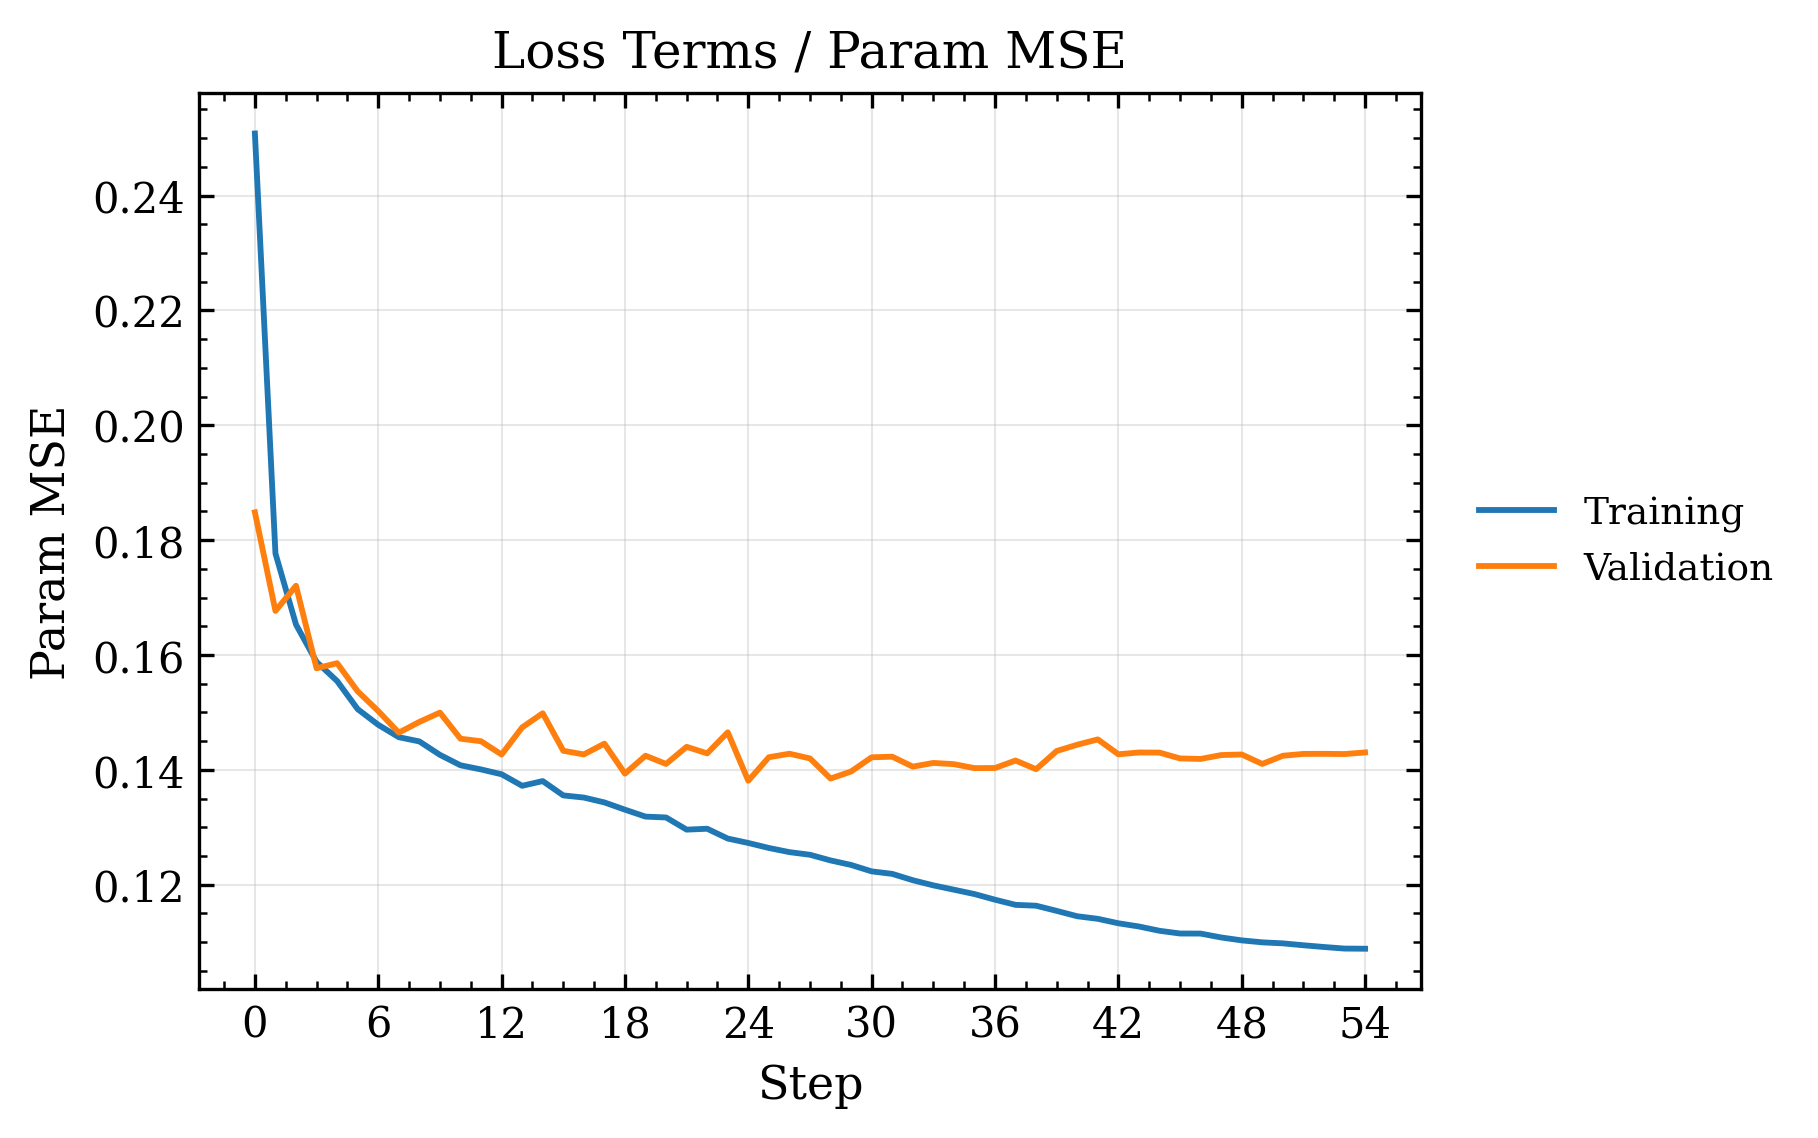
\includegraphics[width=\linewidth]{../figures/K2/augmentation_experiment/param_mse_no_aug.png}\\[3pt]
      {\scriptsize\color{soft} validation flattens early --- training pulls away, the single-scene overfit sets in.}
    \end{column}
    \begin{column}{0.5\textwidth}
      \centering
      {\small\textbf{\textcolor{good}{flips ($p{=}0.5$ each)}}}\\[3pt]
      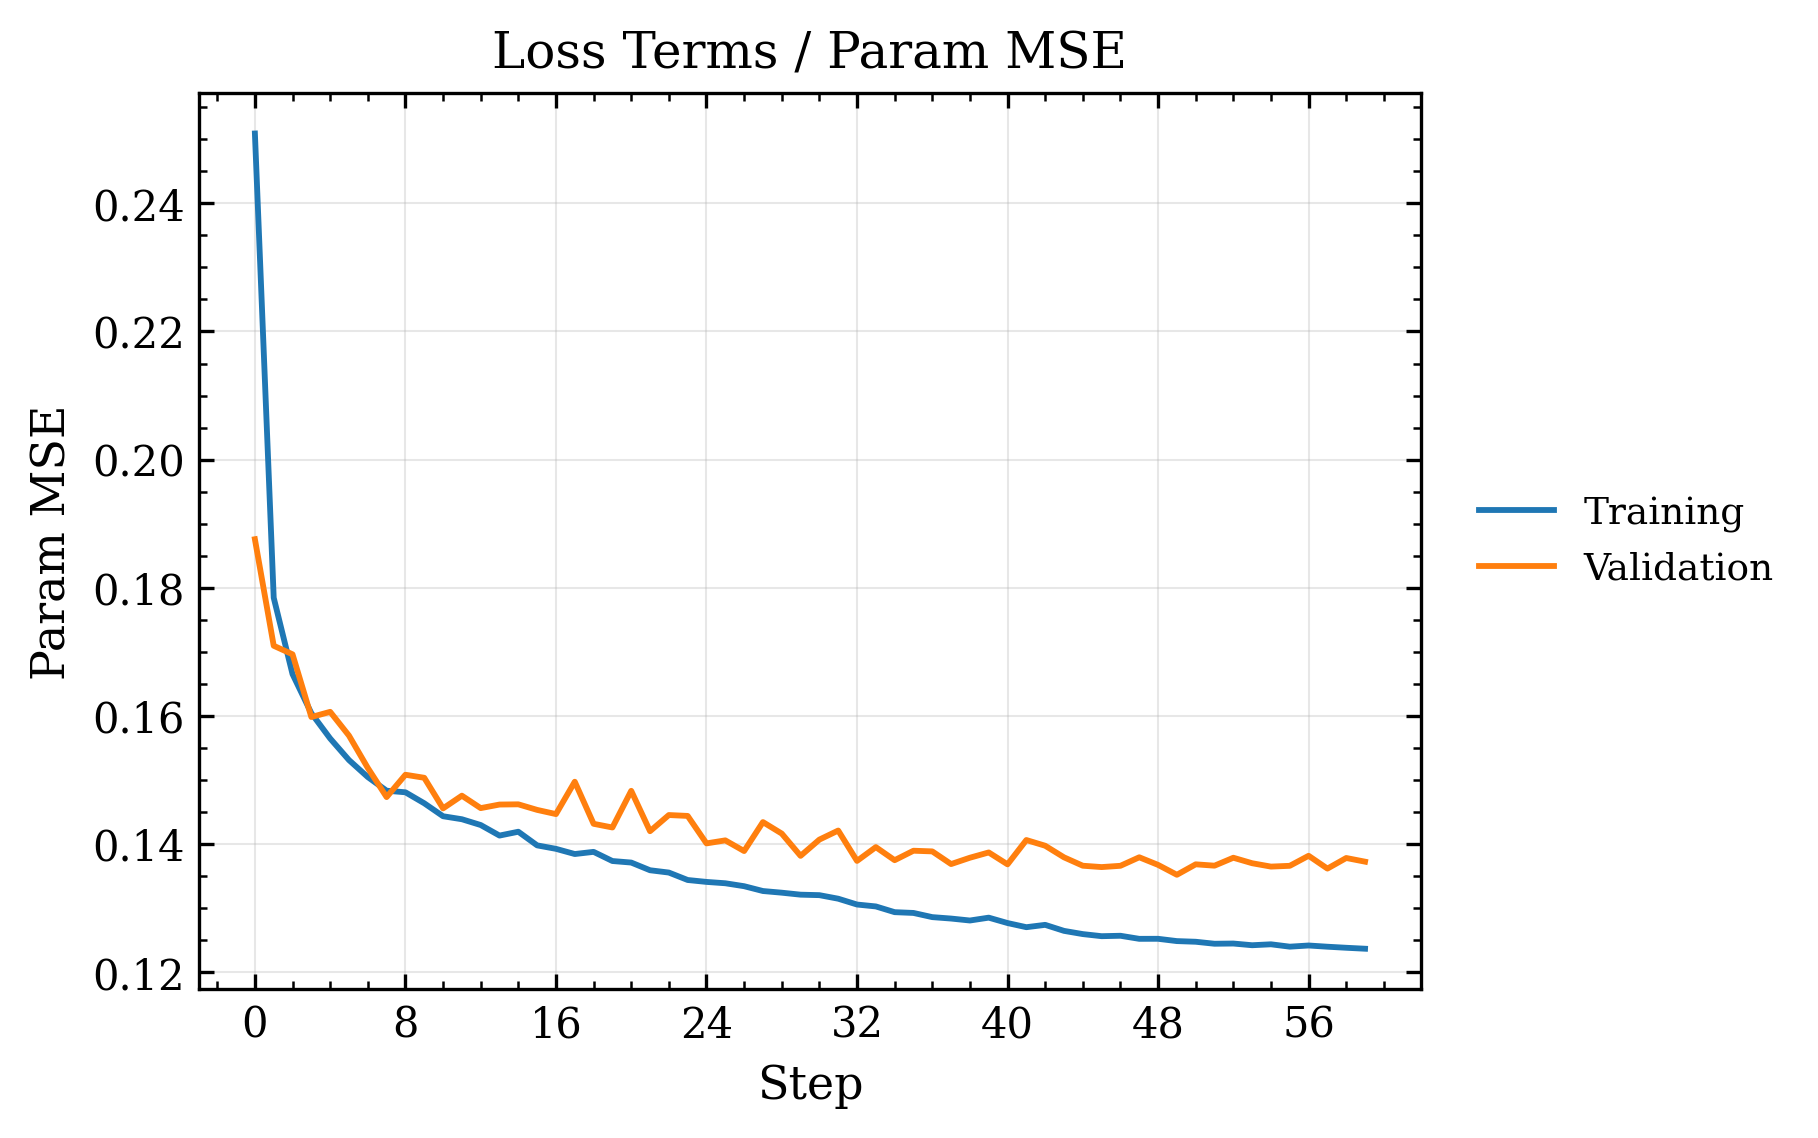
\includegraphics[width=\linewidth]{../figures/K2/augmentation_experiment/param_mse_aug.png}\\[3pt]
      {\scriptsize\color{soft} validation keeps descending --- the train--val gap stays narrow for longer.}
    \end{column}
  \end{columns}
\end{frame}
